%%%%%%%%%%%%%%%%%%%%%%%%%%%%%%%%%%%%%%%%%%%%%%%%%%%%%%%%%%%%%%%%%
% Tese de Doutorado / Dept Fisica, CFM, UFSC                    %
% Andre@UFSC - 2014                                             %
%%%%%%%%%%%%%%%%%%%%%%%%%%%%%%%%%%%%%%%%%%%%%%%%%%%%%%%%%%%%%%%%%

%:::::::::::::::::::::::::::::::::::::::::::::::::::::::::::::::%
%                                                               %
%                          Capítulo 2                           %
%                                                               %
%:::::::::::::::::::::::::::::::::::::::::::::::::::::::::::::::%

%***************************************************************%
%                                                               %
%                         IFS + CALIFA                          %
%                                                               %
%***************************************************************%

\chapter{Síntese de populações estelares em espectroscopia de campo integral}
\label{sec:ifs}

%***************************************************************%
%                                                               %
%                      O survey CALIFA                          %
%                                                               %
%***************************************************************%

\section{O {\em survey} CALIFA}
\label{sec:ifs:califa}

O {\em Centro Astronómico Hispano Alemán} (CAHA) se localiza na {\em Sierra de
los Filabres}, na Comunidade Autônoma de Andaluzia, Espanha. Ele é operado pelo
{\em Max-Planck-Institut für Astronomie} (MPIA), em Heidelberg, Alemanha, e pelo
{\em Instituto de Astrofísica de Andalucía} (IAA/CSIC), em Granada, Espanha. O
{\em survey} CALIFA foi agraciado com 210 noites pelo Comitê Executivo do Calar
Alto, espalhadas por 6 semestres, iniciando em junho de 2010 (na prática, as
observações se estenderam até o final de 2014). O instrumento utilizado foi a
unidade de campo integral PPAK\footnote{{\em PMAS fiber PAcK}.}
\citep{Kelz2006}, do Espectrógrafo PMAS\footnote{{\em Potsdam Multi-Aperture
Spectrophotometer.}} \citep{Roth2005, Roth2010}, no telescópio de
$3,5\,\mathrm{m}$ do CAHA.

A intenção do {\em survey} é caracterizar a população local de galáxias, que
pode ser resumida nos seguintes aspectos científicos principais
\citep{Sanchez2012}:
\begin{itemize}
  \item Amostra cobrindo uma fração substancial da função de luminosidade.
  \item Amostra grande o suficiente para obter conclusões com uma estatística
  significativa para todas as classes de galáxias do {\em survey}.
  \item Caracterização das galáxias sobre toda a sua extensão, evitando bias de
  abertura.
  \item Determinação de mecanismos de ionização do gás: formação estelar,
  choques, AGN.
  \item Medição de abundâncias de oxigênio e nitrogênio no gás ionizado (regiões
  \HII).
  \item Medição de propriedades de populações estelares: idades, razões
  massa-luminosidade, metalicidades e (de forma limitada) padrões de
  abundâncias.
  \item Medição de cinemática galática em gás em estrelas, campos de velocidade
  para todas as galáxias e dispersão de velocidades para as mais massivas.
\end{itemize}
A arquitetura do {\em survey} foi então desenhada levando em conta os
requerimentos acima, junto com as limitações instrumentais e de tempo
disponível. Ela está descrita nas seções a seguir.

\subsection{Instrumentação}
\label{sec:ifs:instrumentacao}

% FIXME: Rogério - Labels em português.

\begin{figure}
	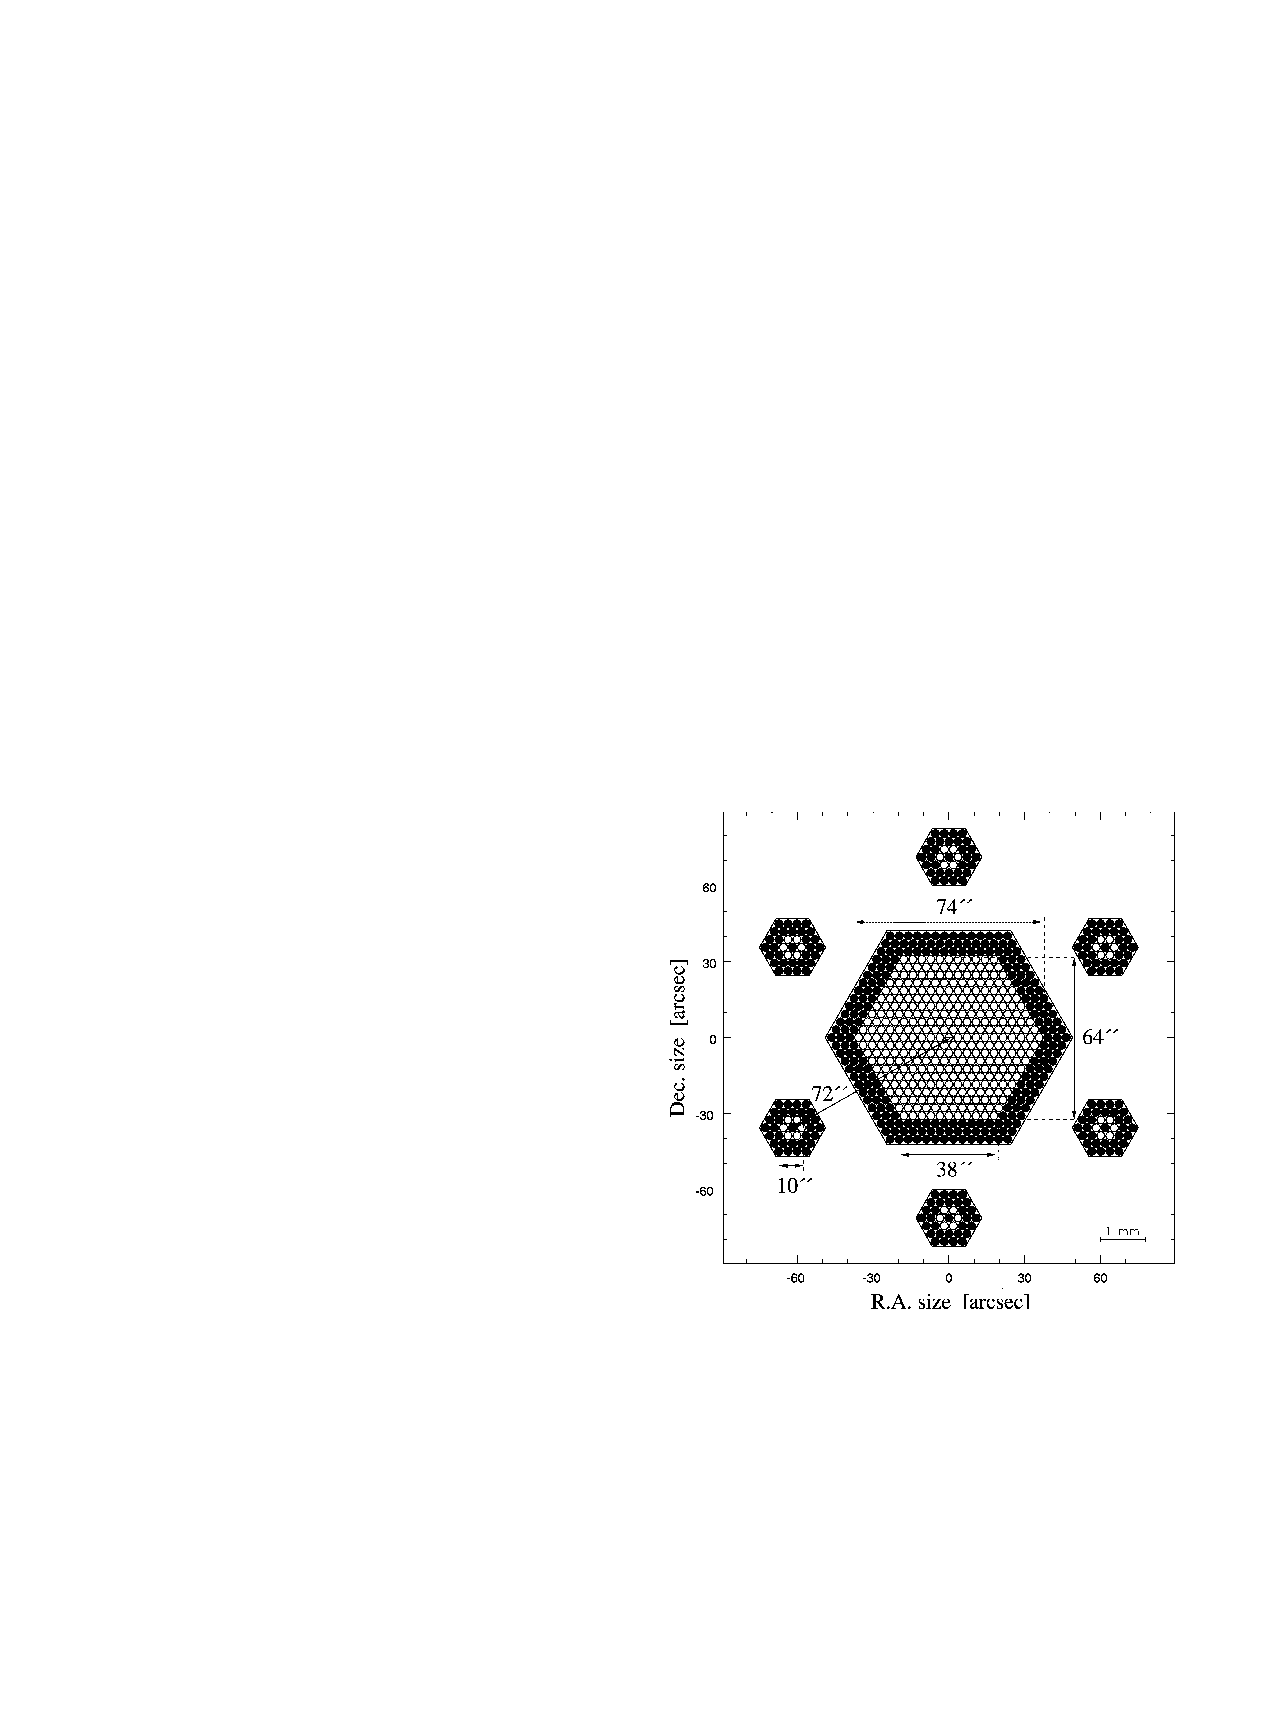
\includegraphics[width=0.5\textwidth]{figuras/PPAK}
	\caption[Distribuição das fibras no instrumento PMAS/PPAK]
	{Distribuição espacial das fibras e dimensões do IFU do instrumento PMAS/PPAK.
	Círculos brancos representam fibras ativas, e círculos pretos fibras
	espaçadoras, que têm apenas papel estrutural e não obtêm espectros. Os 6
	conjuntos de fibras ao redor do IFU são utilizados para medir o céu. O tamanho
	físico é de $4\,\mathrm{mm}$ e a largura do campo é maior que $1\,\arcs$.
	Retirado de	\citet{Kelz2006}.}
	\label{fig:PPAK}
\end{figure}

À época do início do CALIFA\footnote{Hoje em dia o MUSE
(\url{https://www.eso.org/sci/facilities/develop/instruments/muse.html}) é o
detentor do recorde.}, o PPAK/PMAS era o instrumento de sua classe com o maior
tamanho de campo, $>1\,\mathrm{arcmin}^2$. Ele consiste em um maço de 331 fibras
ópticas cobrindo o campo de observação, direcionado a um espectrógrafo de fenda
longa que espalha a luz sobre um detector CCD\footnote{{\em Charge Coupled
Device}.}.
A Figura \ref{fig:PPAK} ilustra a montagem esquemática do instrumento. Desta
forma, de cada fibra se obtém um espectro. Através de um programa de computador,
os espectros podem ser reorganizados de modo a formar um cubo de dados, onde há
duas dimensões espaciais e uma dimensão espectral.
Todavia, pode-se notar na Figura \ref{fig:PPAK} que as fibras não cobrem
totalmente o campo de observação. Na verdade, apenas em torno de 60\% da luz
proveniente do campo cai dentro das fibras. O restante se perde nos espaços
entre elas. Para mitigar este problema utiliza-se uma técnica chamada {\em
dithering}, observando-se o mesmo campo 3 vezes, a cada vez deslocando o
telescópio uma fração do diâmetro de uma fibra em direções diferentes formando
um triângulo, tal que as 3 exposições cobrem toda a àrea a ser observada. O cubo
de dados é reconstruído utilizando os programas de computador da {\em pipeline}
de observação \citep{Sanchez2012}.

\begin{figure}
	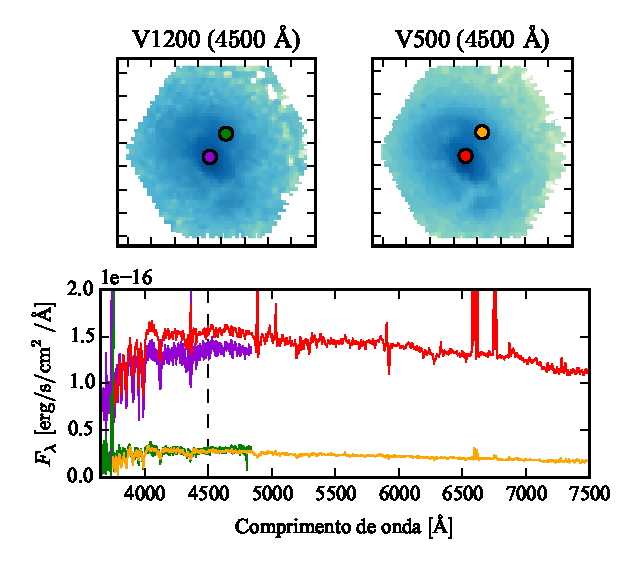
\includegraphics{figuras/DR2_sample_spectra}
	\caption[Exemplos de espectros V500 e V1200 do CALIFA]
	{Espectros V500 e V1200 da galáxia NGC 7625, publicada no DR2 do CALIFA
	\citep{GarciaBenito2015}. Nos painéis superiores são mostradas imagens em
	$4500\,\angstrom$ nas duas configurações. Os espectros referentes aos pontos
	de cores violeta e vermelho, localizados no núcleo, e aos pontos de cores
	verde e laranja, a $12\,\arcs$ do núcleo, são mostrados no painel inferior,
	com as mesmas cores. A linha tracejada mostra o comprimento de onda utilizado
	nas imagens.}
	\label{fig:DR2ExampleSpectra}
\end{figure}

A estratégia inicial do {\em survey} foi observar todos os objetos utilizando
duas configurações diferentes e complementares do instrumento. A primeira
utiliza a grade de difração V500, com resolução $\lambda / \Delta\lambda \approx
850$ em $\lambda = 5000\,\angstrom$ e uma largura a meia altura $\mathrm{FWHM}
\approx 6\,\angstrom$, cobrindo a maior faixa espectral possível, tal que as
linhas \OII e \SII sejam observadas para todos os objetos da amostra.
A segunda utiliza a grade de difração V1200, com resolução $\lambda /
\Delta\lambda \approx 1650$ em $\lambda = 4500\,\angstrom$ e uma largura a meia
altura $\mathrm{FWHM} \approx 2,7\,\angstrom$, cobrindo a faixa azul do
espectro, para incluir a descontinuidade de Balmer, \Hdelta, \Hgamma e
\OIII4363.
Estas duas configurações são chamadas daqui em diante de V500 e V1200
respectivamente. A principal motivação para as observações com a V1200 é medir a
cinemática estelar, explorando a maior resolução espectral dessa grade
($\sigma_{\mathrm{instrumental}} \sim 78\, \mathrm{km}/\mathrm{s}$). Exemplos de
espectros obtidos com as duas configurações, para a galáxia NGC 7625, são
mostrados na Figura \ref{fig:DR2ExampleSpectra}.


\subsection{Amostra}

A amostra obtida pelo CALIFA deve satisfazer os requerimentos científicos
descritos anteriormente, levando em conta as limitações técnicas e
instrumentais. Assim, uma amostra foi inicialmente selecionada a partir do
catálogo DR7 do SDSS \citep{Abazajian2009}, garantindo a disponibilidade de
imagens de boa qualidade em múltiplas bandas espectrais, e, em muitos casos,
espectros nucleares. Sobre esta amostra inicial foram feitos cortes referentes
ao tamanho aparente e o {\em redshift} da galáxia. O tamanho aparente da galáxia
deve ser compatível com o instrumento, por isso escolheu-se limitar a amostra em
diâmetro da isofota de brilho superficial $25\,\mathrm{mag}/\mathrm{arcsec}^2$
($D_{25}$), tal que $45\,\arcs < D_{25} < 80\,\arcs$ na banda $r$ do SDSS. O
{\em redshift} deve ser $0,005 < z < 0,03$, para manter a cobertura espectral
consistente, e também descartar objetos do catálogo que são na verdade estrelas
classificadas como galáxias de forma equivocada.
O resultado é uma amostra de 939 galáxias, denominada {\em amostra mãe},
descrita e estudada em detalhes por \citet{Walcher2014}. O conteúdo da amostra,
junto com tabelas auxiliares, está disponível no {\em website} do
CALIFA\footnote{\url{http://www.caha.es/CALIFA/}}. Todas as galáxias da amostra
têm imagens obtidas nas bandas óptica (SDSS), infravermelha próxima (WISE) e
rádio (NVSS); 655 delas têm fotometria em ultravioleta (GALEX) e 42 têm imagens
em raios-X (Chandra). Espectros ópticos do SDSS DR7 (obtidos a menos de
$15\,\arcs$ do núcleo) estão disponíveis para 622 galáxias da amostra.

A amostra final observada deve conter aproximadamente $2/3$ da amostra mãe, em
torno de 600 galáxias, a serem selecionadas conforme a visibilidade, num padrão
quase aleatório. A Figura \ref{fig:CALIFASample} mostra a distribuição de
magnitude aparente na banda $r$ contra o {\em redshift} da amostra mãe. O
diagrama cor--magnitude pode ser visto na Figura \ref{fig:CALIFACMD}.

\begin{figure}
	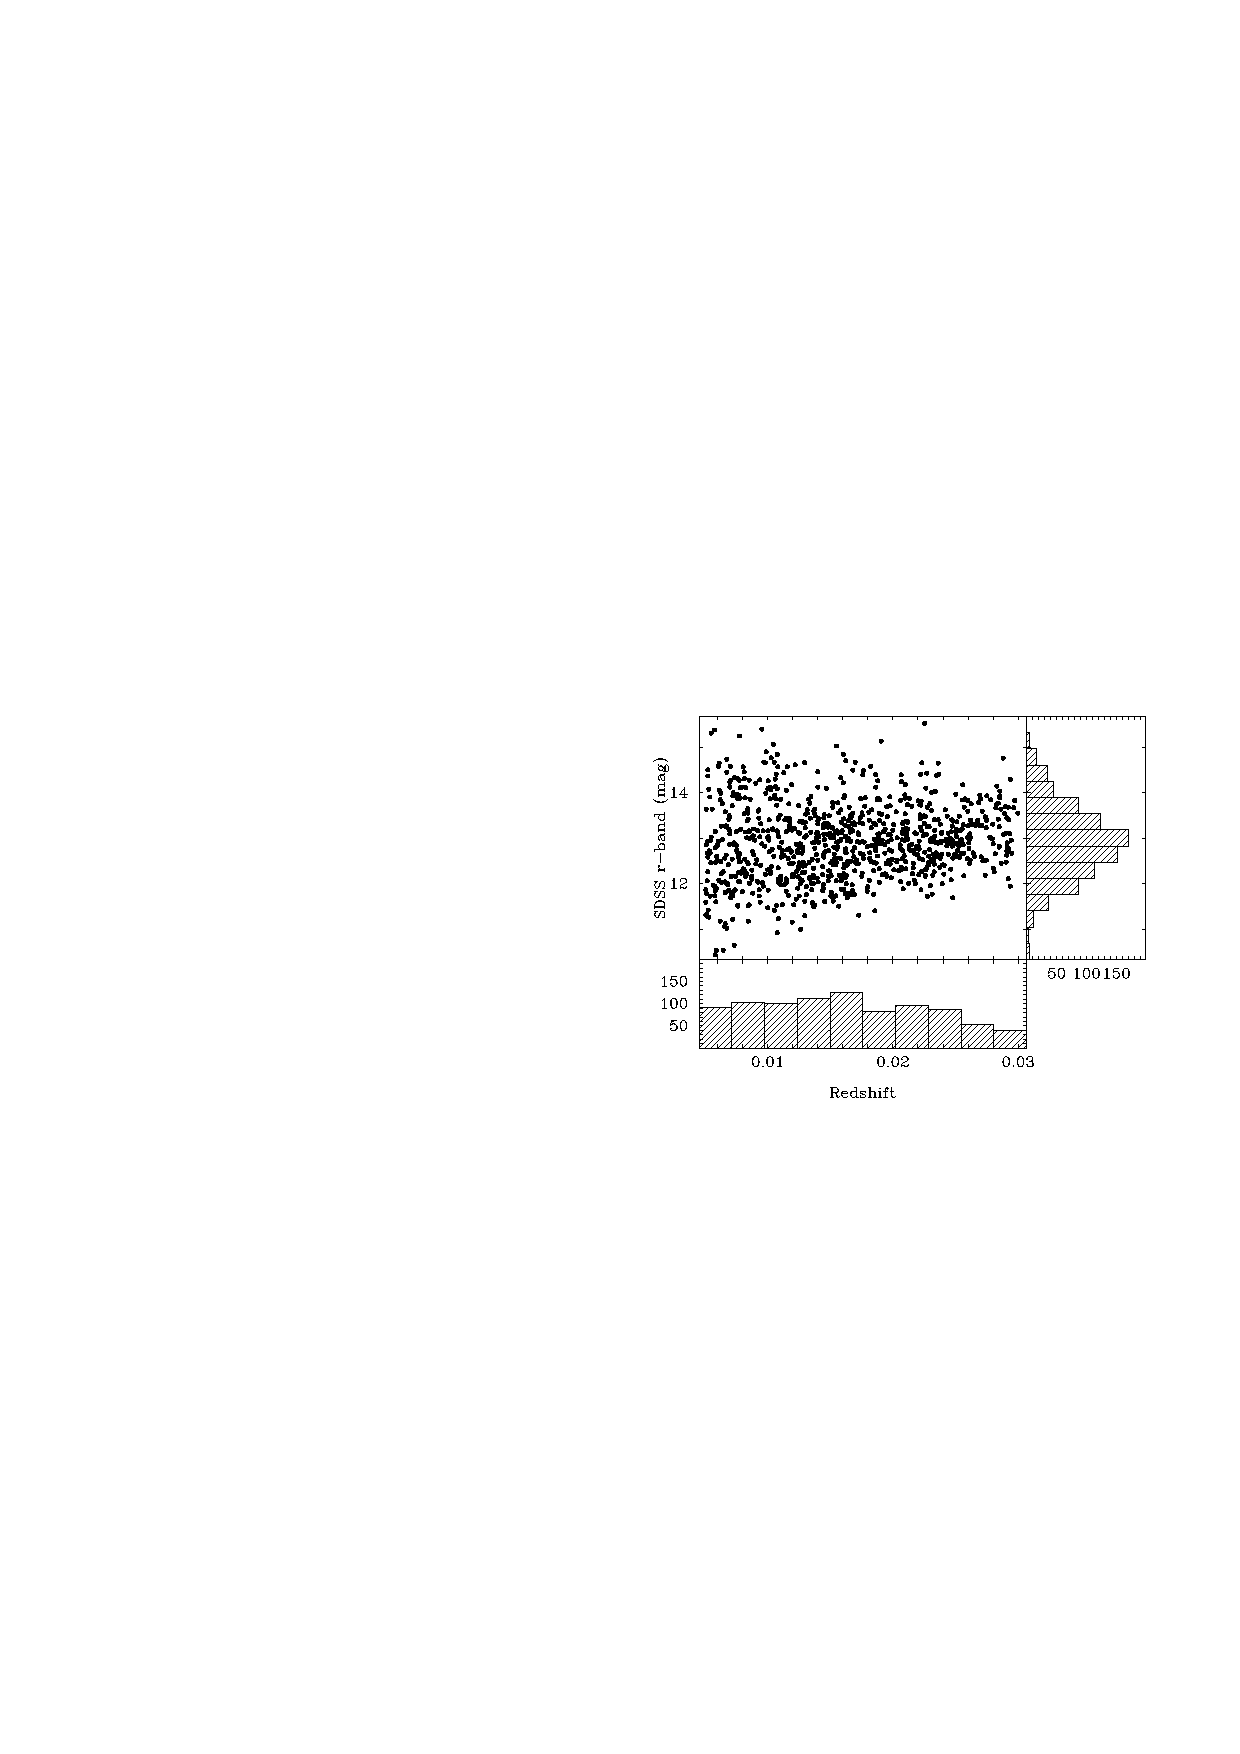
\includegraphics[width=0.7\textwidth]{figuras/CALIFASample}
	\caption[Distribuição de magnitude $r$ contra {\em redshift} da amostra mãe
	do CALIFA] {Distribuição de magnitude aparente na banda $r$ contra o {\em
	redshift} da amostra mãe do CALIFA. Retirado de \citet{Sanchez2012}.}
	\label{fig:CALIFASample}
\end{figure}

\begin{figure}
	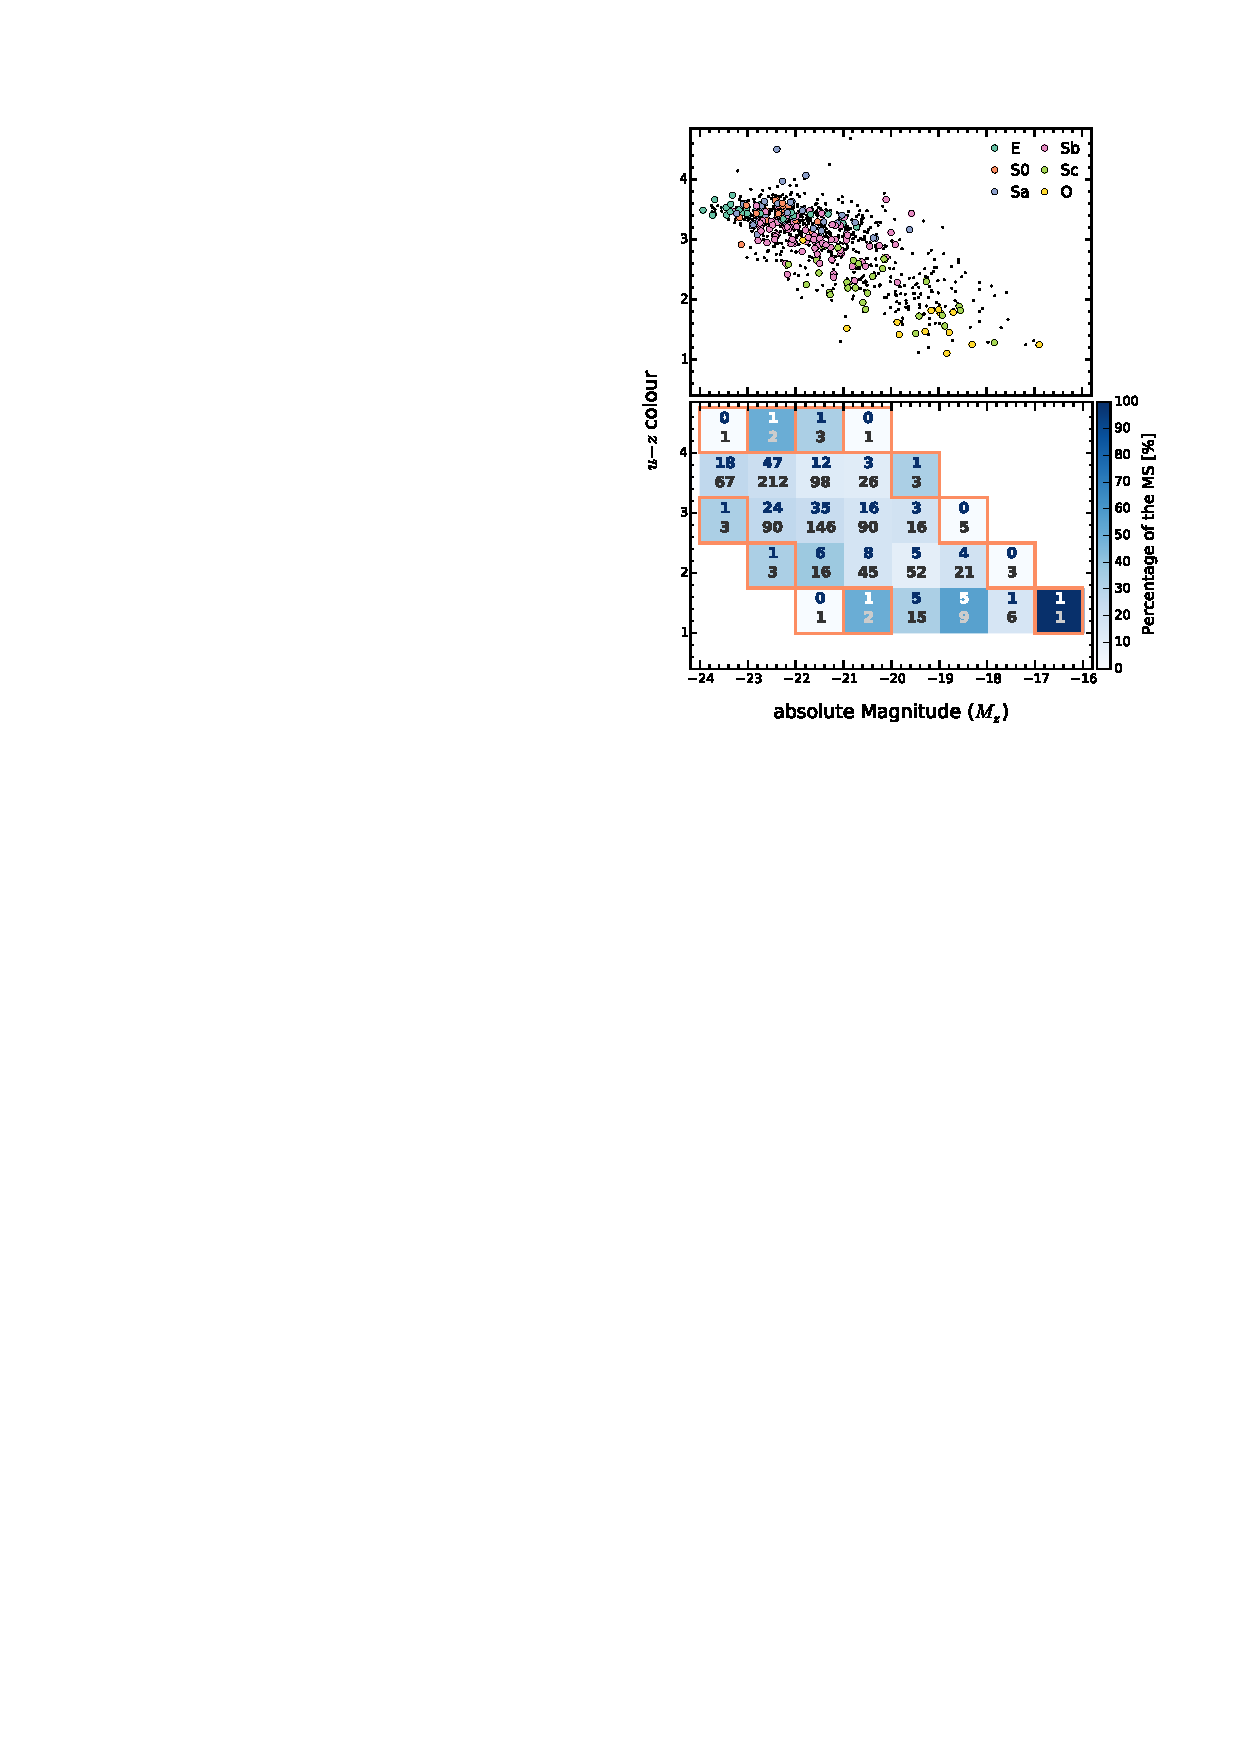
\includegraphics[width=0.7\textwidth]{figuras/CALIFACMD}
	\caption[Diagrama cor--magnitude da amostra mãe do CALIFA]
	{Painel superior: diagrama cor--magnitude ($u-z$ contra $M_z$) da amostra mãe
	do CALIFA. Os círculos coloridos indicam galáxias publicadas no DR2 (ver Seção
	\ref{sec:ifs:dr}), com a cor indicando o tipo morfológico. Painel inferior:
	pecentual das galáxias publicadas no DR2 com respeito à amostra mãe. Os números
	indicam a quantidade observada (cima) e a quantidade na amostra mãe (baixo) em
	cada caixa. Caixas com contornos laranja contém poucas galáxias da
	amostra. Retirado de
	\citet{GarciaBenito2015}.}
	\label{fig:CALIFACMD}
\end{figure}


\subsection{{\em Data Releases}}
\label{sec:ifs:dr}

A primeira liberação pública de dados (em inglês, {\em data release}),
denominada DR1 \citep{Husemann2013}, ocorreu em outubro de 2013. Foram
escolhidas 100 galáxias nas duas configurações, V500 e V1200, que passaram por
um controle de qualidade do {\em survey}, num total de 200 cubos de dados. As
características da amostra do DR1 reproduzem bem as da amostra mãe, dentro do
que é esperado estatisticamente para uma amostra menor.

\begin{figure}
	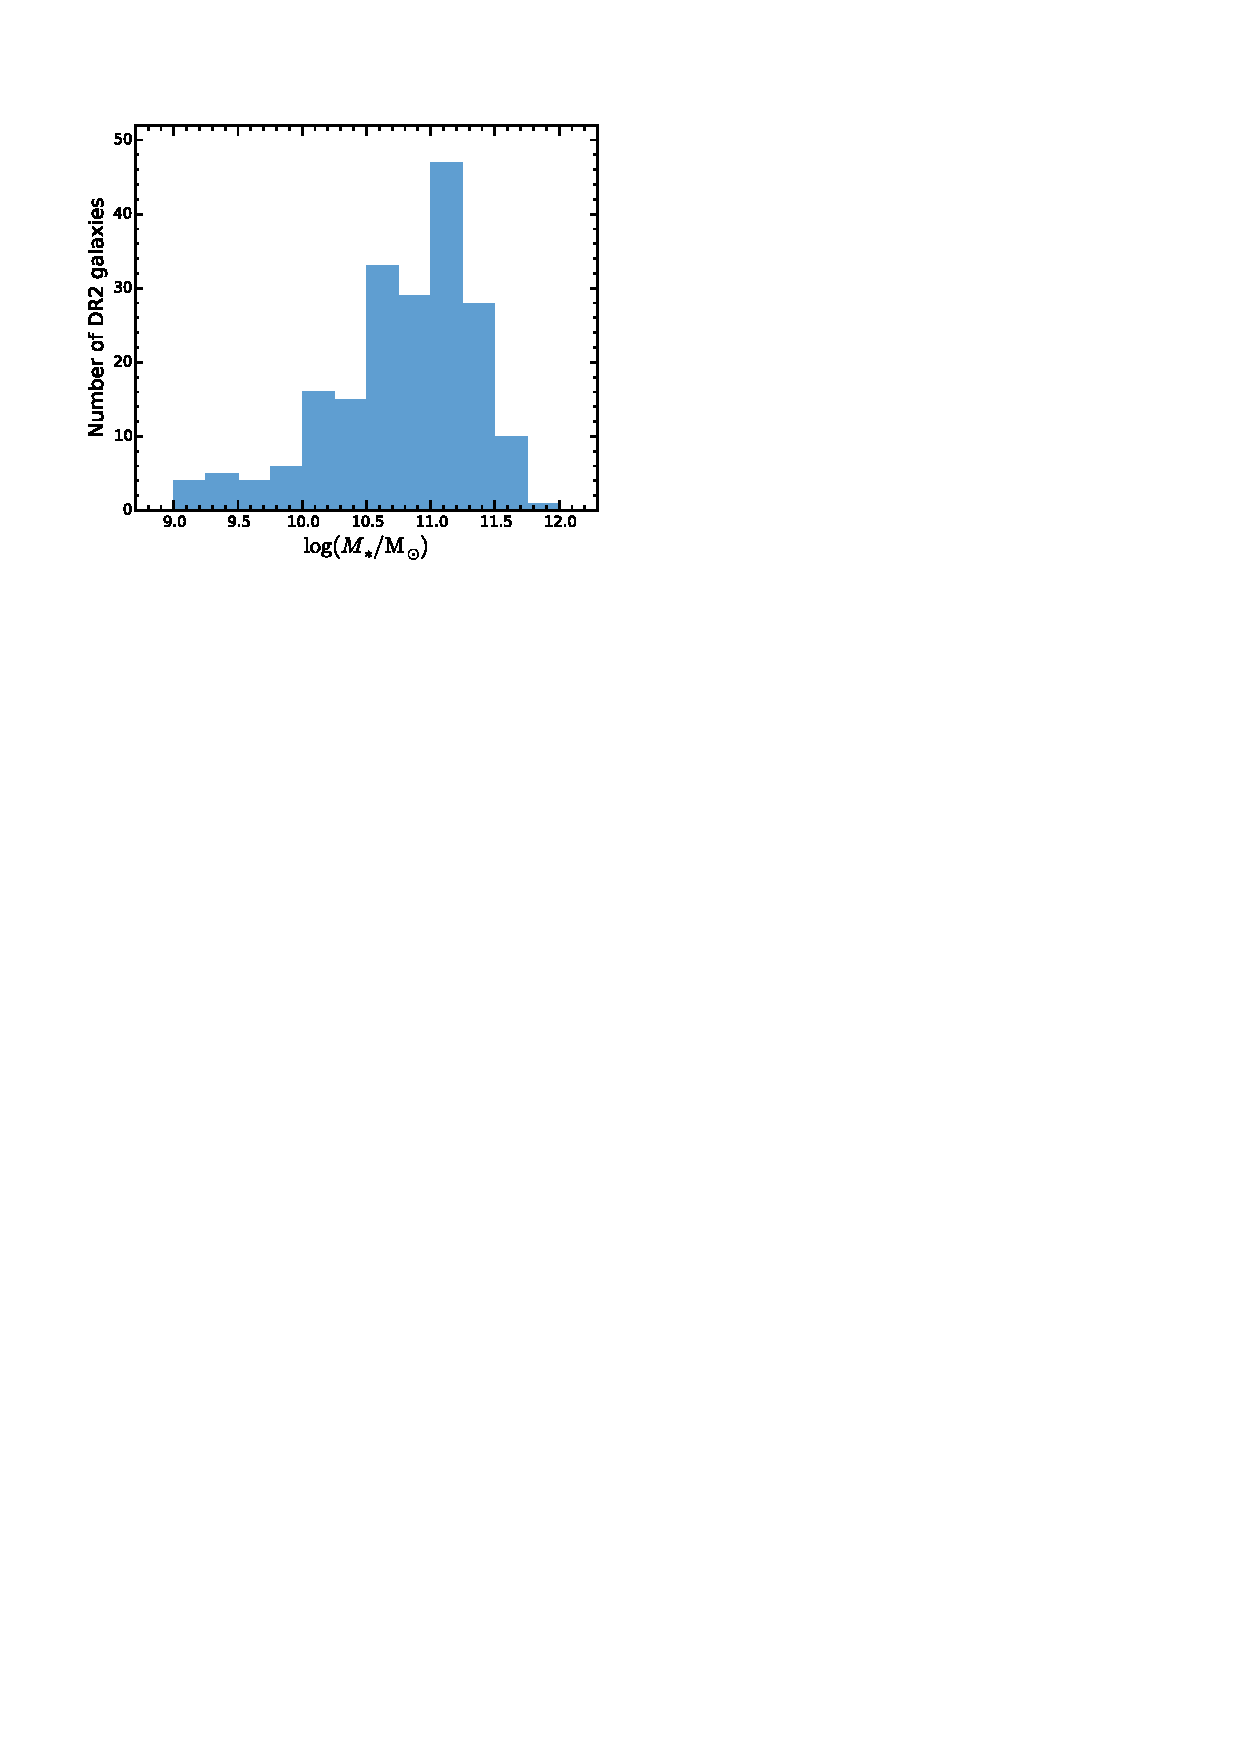
\includegraphics[width=0.5\textwidth]{figuras/CALIFAMass}
	\caption[Distribuição de massa das galáxias no  DR2 do CALIFA]
	{Distribuição de massa estelar das galáxias no DR2 do CALIFA. As massas
	foram determinadas através de síntese espectral de populações estelares com o
	\starlight. Retirado de \citet{GarciaBenito2015}.}
	\label{fig:DRMass}
\end{figure}

\begin{figure}
	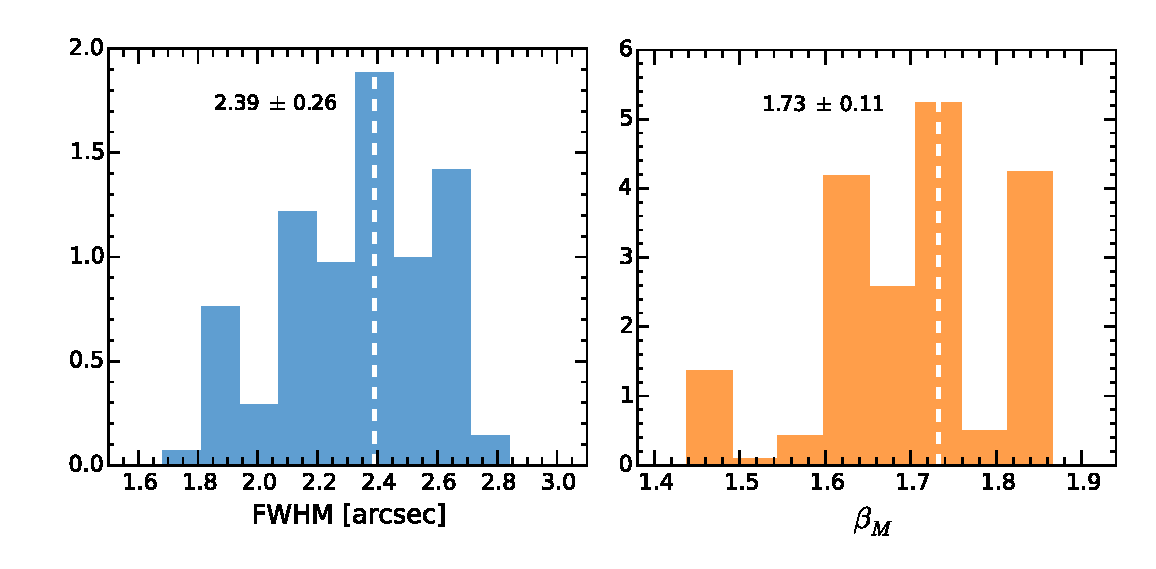
\includegraphics[width=0.8\textwidth]{figuras/DR2PSF}
	\caption[Caracterização da PSF do CALIFA DR2]
	{Caracterização da PSF do CALIFA DR2. À esquerda, distribuição da largura a
	meia altura ($\mathrm{FWHM}$), e à direita, de $\beta$ de um perfil de Moffat.
	Ver mais detalhes na Seção \ref{sec:psf:medida}. Retirado de
	\citet{GarciaBenito2015}.}
	\label{fig:DR2PSF}
\end{figure}

O {\em data release} seguinte, DR2 \citep{GarciaBenito2015}, dobra a quantidade
de cubos de dados, com 200 galáxias nas duas configurações. Todos os cubos de
dados do DR2 foram reduzidos com uma versão aprimorada do {\em pipeline} de
redução de dados, apresentando melhor calibração espectrofotométrica, registro
de imagem e resolução espacial. A massa das galáxias obtidas através de síntese
espectral de populações estelares foi utilizada para caracterizar a amostra do
DR1 e do DR2 (painel inferior da Figura \ref{fig:DRMass}).
A PSF ({\em Point Spread Function}) típica dos cubos de dados (Figura
\ref{fig:DR2PSF}) do {\em survey} foi determinada utilizando as mesmas técnicas
de ajuste de imagem apresentadas no Capítulo \ref{sec:Decomp}. Mais detalhes
sobre a medição da PSF no Capítulo \ref{sec:psf}. Um {\em data release} final
está programado para o final de 2015.


%***************************************************************%
%                                                               %
%                      O survey CALIFA                          %
%                                                               %
%***************************************************************%
\section{Síntese de população estelar}
\label{sec:ifs:sintese}

% FIXME: Rogério - Esta seção deveria vir primeiro e iniciar pelo starlight.

\subsection{\textsc{qbick}}
\label{sec:ifs:qbick}

O programa \textsc{qbick} foi desenvolvido por Rubén García Benito para fazer o
mascaramento e tesselação dos cubos de dados descrito a seguir. Para mais
detalhes sobre o processo completo, ver o artigo por \citet{CidFernandes2013},
reproduzido no Apêndice \ref{apendice:PaperResolving1}.

É preciso preparar os espectros para passarem pelo \starlight. Isto envolve
principalmente remover medidas não confiáveis, além de deixar todos os espectros
e cubos de dados num formato comum, para executar o \starlight em modo {\em
pipeline}. Antes de tudo, todos os {\em spaxels} que contêm luz não proveniente
da galáxia, como estrelas de campo ou galáxias de fundo, foram mascarados.
Também foram mascarados artefatos da observação e regiões de baixo sinal--ruído.
Este é um procedimento quase artesanal, e necessita de um bom par de vistas
humanas bem treinadas. Para um {\em survey} do porte do CALIFA, com cerca de 600
galáxias, isto ainda é factível. Após o mascaramento espacial, foram mascaradas
as linhas espectrais causadas pela atmosfera terrestre. Os espectros foram em
seguida postos no referencial de repouso utilizando o {\em redshift} obtido pela
{\em pipeline}, medido nos $5\,\arcs$ centrais da galáxia. Foi escolhida uma
janela espectral de $5590$ a $5680\,\angstrom$ para fazer a medida do
sinal--ruído dos espectros. Espectros com sinal--ruído baixo, em geral nas
regiões menos brilhantes da galáxia, podem gerar resultados espúrios no
\starlight. Estes espectros foram combinados de modo a obter um melhor
sinal--ruído utilizando uma técnica conhecida como tesselação de Voronoi. Foi
escolhido um sinal--ruído de 20 como alvo para o agrupamento dos {\em spaxels}.
O código utilizado para a tesselação de Voronoi foi implementado por
\citet{Cappellari2003} e modificado para levar em conta erros correlacionados.
Um exemplo de aplicação do \textsc{qbick} é mostrado na Figura \ref{fig:QBICK}.

\begin{figure}
	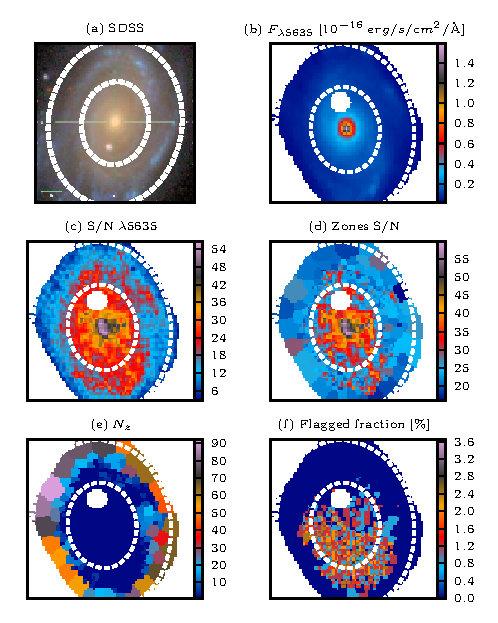
\includegraphics[width=0.8\textwidth]{figuras/zones-K0277}
	\caption[Exemplo processamento com \textsc{qbick}, galáxia K0277]
	{Exemplo processamento com \textsc{qbick} da galáxia NGC 2916 (CALIFA 0277). (a)
	Imagem do SDSS na banda $r$. (b) Imagem do CALIFA em $5635\,\angstrom$ com máscara
	espacial. (c) Mapa de sinal--ruído em $5635\,\angstrom$. (d) Sinal--ruído após
	a segmentação em zonas de Voronoi. (e) Número de {\em spaxels} em cada zona.
	(f) Percentual de {\em pixels} ruins na faixa de $3800$--$6850\,\angstrom$.
	Retirado de \citet{CidFernandes2013}.}
	\label{fig:QBICK}
\end{figure}

\subsection{\starlight}
\label{sec:ifs:starlight}

O \starlight é um código de síntese espectral desenvolvido por
\citet{CidFernandes2005}. Nele, o espectro observado de uma galáxia é modelado
como uma combinação linear de espectros de uma base, um modelo de atenuação por
poeira, e efeitos cinemáticos ({\em redshift} e dispersão gaussiana de
velocidades). Esta base é composta por uma grade de populações estelares simples
(SSP), onde cada SSP consiste em um conjunto de estrelas formadas ao mesmo tempo
com a mesma metalicidade, com espectros proveniente de alguma biblioteca de
modelos. O \starlight busca neste espaço de parâmetros (que pode ser imenso, com
quase 300 dimensões no caso do presente estudo) qual conjunto de frações de luz,
atenuação e cinemática que melhor ajusta o espectro observado, que toma a forma
\begin{equation*}
F^{\mathrm{modelo}}_\lambda = \sum_{j=1}^{N_\star} F^\star_\lambda(t_j,Z_j)
10^{ -0,4 A_\lambda}  \otimes G(v_\star,\sigma_\star).
\end{equation*}	
Nesta equação, $F^{\mathrm{modelo}}_\lambda$ é o fluxo em cada comprimento de
onda. O termo $10^{ -0.4 A_\lambda}$ corrige o espectro pelo efeito de atenuação
interestelar, que pode ser por exemplo do tipo CCM \citep*{Cardelli1989} ou
CAL \citep*{Calzetti1994}. $G(v_\star,\sigma_\star)$ denota uma função
gaussiana (centrada em $v_\star$ e com dispersão $\sigma_\star$) utilizada para
modelar os efeitos da cinemática estelar. Na prática a equação acima é
implementada após um procedimento de normalização a um comprimento de onda de
referência $\lambda_N$, isto é,
\begin{equation*}
F^{\mathrm{modelo}}_\lambda = F^{\mathrm{modelo}}_{\lambda_N} 
\sum_{j=1}^{N_\star} x_j b^\star_\lambda(t_j,Z_j)
10^{ -0,4 (A_\lambda - A_{\lambda_N}) } \otimes G(v_\star,\sigma_\star),
\end{equation*}
onde $b^\star_\lambda(t_j,Z_j) \equiv  F^\star_\lambda(t_j,Z_j) /
F^\star_{\lambda_N}(t_j,Z_j)$ denota o espectro  do elemento $j$ da base
normalizado a seu valor em $\lambda_N$. A dada elemento $j$ corresponde uma
idade  $t_j$ e uma metalicidade $Z_j$, e a importância de cada elemento na soma
total é dada pelo peso $x_j$. O conjunto $\{x_j, i=1,2,\ldots,N_\star\}$ é
chamado vetor de população ($\vec{x}$) da galáxia considerada.
O melhor ajuste é escolhido minimizando
\begin{equation*}
\chi^2 = \sum_\lambda \left[(F^{\mathrm{observado}}_\lambda -
F^{\mathrm{modelo}}_\lambda) w_\lambda\right]^2
\end{equation*}
onde o peso $w_\lambda$ é definido como o inverso da incerteza na medida de
$F_\lambda^{\mathrm{observado}}$.

Os espectros da base provêm de modelos de síntese evolutiva de populações
estelares. A maior parte dos resultados publicados do \starlight usa os modelos
de \citet[BC03]{Bruzual2003}. Em particular, em seus estudos de galáxias do SDSS
o grupo da UFSC normalmente usa uma base composta de 150 SSPs cobrindo 25 idades
(entre $0,001$ e $18\,\mathrm{Ga}$) e 6 metalicidades ($\log Z/Z_\odot$ entre
$-2,3$ e $+0,4$; vide \citet{Mateus2006}). A Figura
\ref{fig:StarlightSpectrumSample} mostra ajustes feitos para 5 galáxias do SDSS
utilizando esta base. A extinção é modelada com uma lei de avermelhamento de
CCM. Neste trabalho usamos modelos mais atualizados de espectros de SSPs,
extraídos dos modelos de Granada \citep[para idades até
$63\,\mathrm{Ma}$]{GonzalezDelgado2005} e os do projeto MILES \citep[para idades
maiores que $63\,\mathrm{Ma}$]{Vazdekis2010}. No total esta nova base contém 235
elementos cobrindo idades de  $0,001$ a $14\,\mathrm{Ga}$, e $\log Z/Z_\odot$ de
$-2,3$ a $+0,33$.
Para mais detalhes ver \citet{GonzalezDelgado2014b, GonzalezDelgado2014a}.

\begin{figure}
	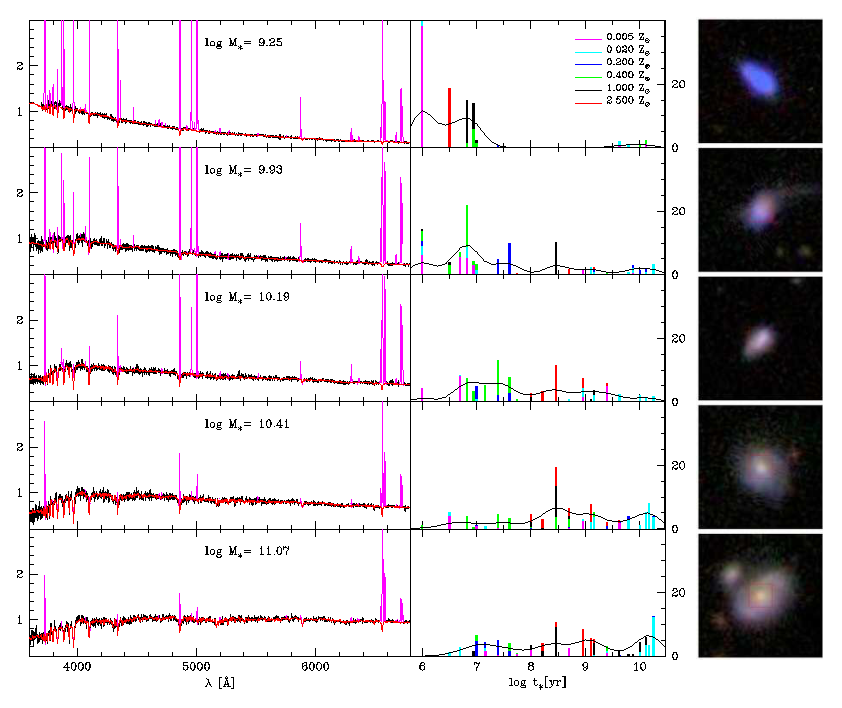
\includegraphics[width=1.0\textwidth]{figuras/starlight-fit}
	\caption[Exemplos de ajuste de espectro com o \starlight]
	{Exemplos de ajuste de espectros de galáxias com o \starlight
	\citep{Asari2007}. À esquerda, espectros observados (preto), espectros
	modelados (vermelho), com regiões mascaradas em magenta. No meio, a fração da
	luz associada a cada uma das 25 idades das SSPs usadas na síntese, com a curva
	representando a versão suavizada do histórico de formação estelar. À direita,
	imagens do SDSS correspondentes às galáxias.}
	\label{fig:StarlightSpectrumSample}
\end{figure}

% FIXME: Rogério - Figura manjada, tu não tens umas tuas?

A aplicação mais imediata do resultado do \starlight é a remoção do contínuo
estelar para medir com maior precisão as linhas de emissão provenientes do gás,
não incluídas no modelo. É possível também estudar o vetor de população
$\vec{x}$, que representa a fração de luz proveniente de cada população estelar
da base (como na coluna central de painéis da Figura
\ref{fig:StarlightSpectrumSample}). De forma alternativa, pode-se utilizar o
vetor de fração de massa $\vec{\mu}$, que se relaciona ao $\vec{x}$ através da
relação massa--luminosidade de cada elemento da base. Individualmente os
componentes $x_j$ e $\mu_j$ dos vetores não são confiáveis, pois há muita
degenerescência nos elementos da base \citep{CidFernandes2005}. Porém, a
informação contida nos vetores pode ser condensada, gerando medidas físicas mais
robustas. A idade estelar média ponderada pela luminosidade pode ser definida
como $\langle \log t \rangle_{\mathrm{L}} = \sum_j x_j \log t_j$, onde $t_j$ é a
idade de cada elemento da base.
Pode-se substituir o vetor de população ($\vec{x}$) pelo vetor de fração de
massa ($\vec{\mu}$) e assim obter a idade ponderada pela massa. Outra
propriedade bastante utilizada é a metalicidade estelar média ponderada pela
massa, definida como $\langle Z \rangle_{\mathrm{M}} = \sum_j \mu_j Z_j$, onde
$Z_j$ é a metalicidade de cada elemento da base. Medidas como estas geram
resultados muito mais confiáveis, como demonstrado por \citet{CidFernandes2014},
reproduzido no Apêndice \ref{apendice:PaperResolving1}.

Esta técnica foi utilizada em diversos artigos. Em particular a colaboração
SEAGal ({\em Semi Empirical Analysis of Galaxies}), liderada pela UFSC, aplicou
o \starlight a 926246 espectros de galáxias do DR7 do SDSS. As propriedades
físicas derivadas desta análise de populações estelares, junto com as medidas de
linhas de emissão, foram disponibilizadas como um banco de dados no {\em
website} \url{http://www.starlight.ufsc.br/}.

Os resultados foram utilizados em estudos varrendo desde a história de formação
estelar de galáxias \citep{Asari2007} a efeitos ambientais \citep{Mateus2007} e
a origem de linhas de emissão de galáxias ``aposentadas'' \citep{Stasinska2008,
CidFernandes2011}. Além desses, pesquisadores em todo o mundo produziram artigos
independentes \citep[para citar alguns]{Bian2006, Liang2007, Peeples2009,
Lara-Lopez2009, Lara-Lopez2010} baseados nesse banco de dados.

Em todos esses estudos, cada galáxia é representada por apenas um espectro. A
extensão desse tipo de estudo a dados IFS parece trivial, e em certa medida o é
se considerarmos o espectro de cada zona (ou {\em spaxel}) como o espectro de
uma galáxia inteira. No entanto, para tirar máximo proveito da informação sobre
populações estelares e sua distribuição espacial é necessária uma ferramenta que
organize os resultados do \starlight para um dado cubo de dados. Dessa
necessidade nasceu a plataforma \pycasso, assunto do próximo capítulo.

% FIXME: Rogério - Sugestões:
%
% * Separar em dois capítulos.
% * Falar um pouco do histórico de aplicaação do starlight (no RS e em SP tem
% trabalhos com isso).

% End of this chapter

